% ============================================================
%  Chapter 4 — Proposed Methodology
% ============================================================
\chapter{Proposed Methodology: DRL-LSTM-LBRO}
\label{chap:methodology}
\label{chap:sysmodel}

This chapter presents the system model, design, algorithmic construction, and
training procedure of the DRL-LSTM-LBRO framework. The framework
extends the original LBRO heuristic by replacing its static
Composite Resource Index with a learned scheduling policy that
fuses near-future load predictions from a per-cloudlet GRU-LSTM
predictor with real-time resource observations. The resulting
state representation is consumed by a Double Deep Q-Network
(DDQN) agent that is trained end-to-end to minimise task drops,
latency, energy, and load imbalance simultaneously.

% ─────────────────────────────────────────────────────────
\section{System Model}
\label{sec:sysmodel}

\subsection{Three-Tier Network Topology}

The deployment environment follows a three-tier hierarchy.
The \emph{IoT device tier} consists of resource-constrained
sensors, actuators, and mobile clients that continuously
generate computational tasks and cannot process them locally.
The \emph{edge cloudlet tier} comprises $N$ heterogeneous
multi-server nodes deployed at network access points, each
modelled as an M/M/$c$ queue with finite buffer of size $K_i$.
The \emph{cloud tier} is a single data centre modelled as
an M/M/$\infty$ server, reachable over a WAN link with fixed
propagation delay $d_{\text{cloud}}^{\text{prop}} = 50$\,ms.
Figure~\ref{fig:network_topology} illustrates this three-tier
deployment model.

\begin{figure}[ht]
  \centering
  \includegraphics[width=0.85\textwidth]{fig_network_topology.png}
  \caption{Three-tier IoT--Edge--Cloud network topology.
           IoT devices (smart offices, homes, and mobiles) connect
           via access points to edge servers at the edge layer,
           which in turn fall back to a cloud data centre over
           the Internet when local resources are exhausted.}
  \label{fig:network_topology}
\end{figure}

\subsection{IoT Task Model}

Each arriving task $\tau$ is characterised by a tuple
$\langle \text{MI}, r_\tau, d_\tau \rangle$: its computational
demand in millions of instructions (MI $\sim$ Poisson with
mean 500), its RAM requirement $r_\tau$ (drawn from
$\mathcal{U}[256, 1280]$\,MB), and a soft deadline $d_\tau$.
A task assigned to cloudlet $i$ is accepted only if
$q_i(t) < K_i$ and the remaining RAM can accommodate $r_\tau$;
otherwise it is dropped and penalised.

\subsection{Queuing Delay Model}

Each cloudlet is modelled as an M/M/$c$ queue — Poisson arrivals
and exponential service times — as an analytically tractable
approximation. This is a standard assumption in MEC literature
that provides closed-form queueing expressions; the Google Borg
trace distributions are used for task demand parameters rather
than service-time distributions, so the approximation
remains practically grounded.

For a cloudlet with $c_i$ servers and traffic intensity
$\rho_i = \lambda / (c_i \mu_i)$, the expected queueing wait
is given by the Erlang-C formula:
\begin{equation}
  W_i = \frac{C(c_i, \rho_i)}{c_i\,\mu_i\,(1-\rho_i)},
  \quad
  C(c_i,\rho_i) =
  \frac{(c_i\rho_i)^{c_i} / [c_i!(1-\rho_i)]}
       {\sum_{k=0}^{c_i-1}(c_i\rho_i)^k/k!
        +(c_i\rho_i)^{c_i}/[c_i!(1-\rho_i)]}
  \label{eq:erlang_method}
\end{equation}
Total end-to-end latency for a task at cloudlet $i$ is
$l_i = d_i^{\text{prop}} + W_i + \text{MI}/M_i$.

% ─────────────────────────────────────────────────────────
\section{System Architecture Overview}
\label{sec:overview}

The DRL-LSTM-LBRO system is built on a broker-enabled federated
cloudlet paradigm. A central broker maintains real-time knowledge
of every edge node's resource state and makes placement decisions
for each arriving IoT task. The architecture has three functional
layers: (1) the \emph{edge infrastructure layer} comprising
heterogeneous cloudlets and a cloud fallback; (2) the
\emph{prediction layer} containing per-cloudlet GRU-LSTM models
that forecast imminent CPU and RAM utilisation; and (3) the
\emph{decision layer} housing the DDQN scheduling agent.
Figure~\ref{fig:system_arch} shows the main components and their
interconnections.

\begin{figure}[ht]
  \centering
  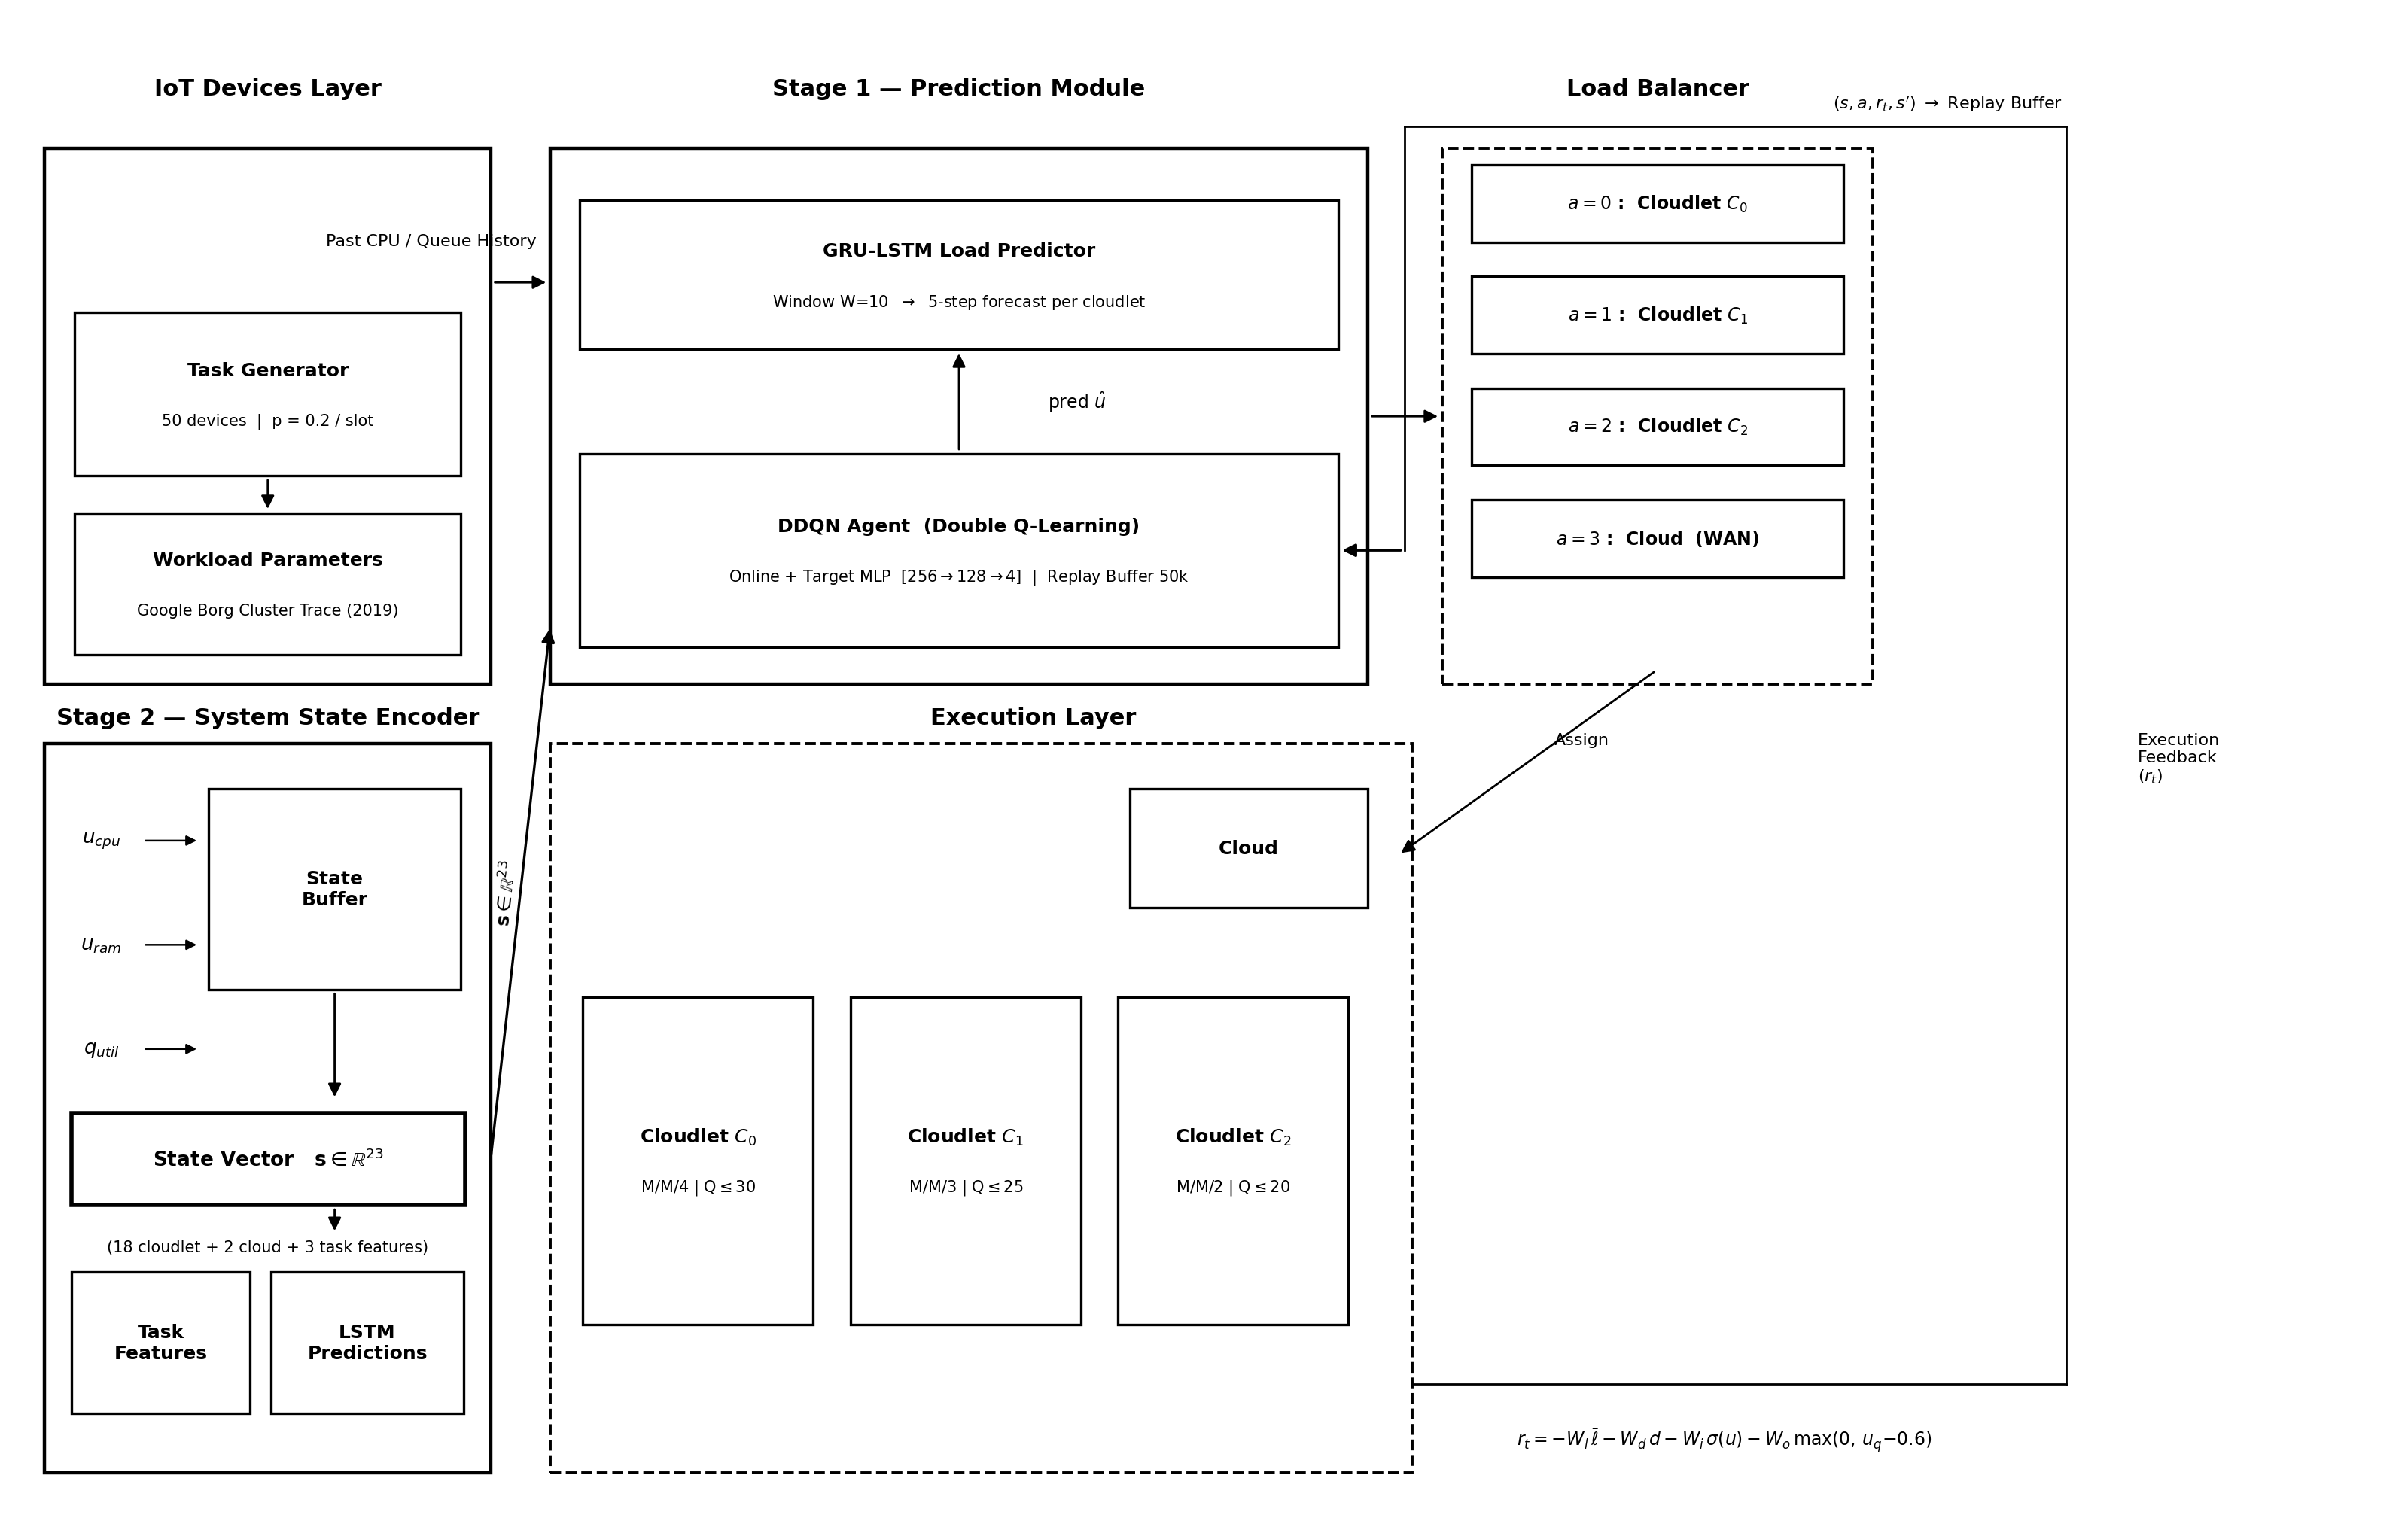
\includegraphics[width=0.85\textwidth]{fig_architecture1.png}
  \caption{DRL-LSTM-LBRO System Architecture: IoT device layer feeds
           tasks to the broker, which uses the GRU-LSTM Prediction
           Module and the DDQN agent to place tasks across three edge
           cloudlets or the cloud fallback.}
  \label{fig:system_arch}
\end{figure}

The pipeline operates as follows: (1) a GRU-LSTM model per
cloudlet forecasts near-future CPU and RAM utilisation from a
sliding window of recent observations; (2) the DDQN agent
constructs its state vector from current resource readings,
LSTM predictions, and the arriving task's feature vector; (3) the
agent selects a placement action; (4) the environment executes the
placement, updates resource utilisations, and returns a scalar
reward; and (5) the agent stores the transition in a replay buffer
and updates its weights via mini-batch gradient descent.

% ─────────────────────────────────────────────────────────
\section{Edge Infrastructure and Simulation Environment}
\label{sec:infra}

The simulation models three heterogeneous edge cloudlets and a
remote cloud fallback, calibrated to represent realistic IoT edge
deployments. Table~\ref{tab:edge_config} summarises the node
parameters.

\begin{table}[htbp]
\centering
\caption{Simulated Edge Cloudlet Configuration}
\label{tab:edge_config}
\renewcommand{\arraystretch}{1.15}
\begin{tabular}{lcccc}
\toprule
\textbf{Node} & \textbf{MIPS} & \textbf{RAM (MB)} &
\textbf{Servers ($c_i$)} & \textbf{Queue Limit ($K_i$)} \\
\midrule
Cloudlet 1 & 8{,}000 & 16{,}384 & 4 & 30 \\
Cloudlet 2 & 8{,}000 & 8{,}192  & 3 & 25 \\
Cloudlet 3 & 8{,}000 & 4{,}096  & 2 & 20 \\
Cloud      & 32{,}000 & $\infty$ & $\infty$ & $\infty$ \\
\bottomrule
\end{tabular}
\end{table}

CPU heterogeneity in queue depth and RAM reflects real-world
diversity across small-board computers, micro-servers, and
gateway appliances. The cloud is modelled as an M/M/$\infty$
server with a fixed WAN propagation delay of 50\,ms. Nodes
communicate over a LAN with propagation delays of 2--4\,ms per
cloudlet. The simulation is implemented in Python using a custom
discrete-event engine; one episode comprises $T = 2{,}000$ time
steps.

% ─────────────────────────────────────────────────────────
\section{Stage 1: GRU-LSTM Load Predictor}
\label{sec:lstm}

\subsection{Motivation for Predictive State Augmentation}

Existing DRL schedulers observe only the current resource state.
Because edge cloudlets operate as M/M/$c$ queues, tasks accepted
at step $t$ continue consuming CPU and RAM for several subsequent
steps. A cloudlet that reports low utilisation at $t$ may already
be trending toward saturation by $t{+}3$. Providing the DDQN
agent with short-horizon forecasts in its state vector allows it
to act proactively rather than reactively.

\subsection{Predictor Architecture}

A separate GRU-LSTM network is trained for each cloudlet. The
input is a sliding window of the last $L = 10$ observed
$(\text{cpu\_util}, \text{ram\_util})$ pairs, forming a sequence
tensor $\mathbf{X} \in \mathbb{R}^{L \times 2}$. The network
architecture is:

\begin{enumerate}
  \item A GRU layer with $H_1 = 32$ hidden units that captures
  short-term local fluctuations in utilisation.
  \item An LSTM layer with $H_2 = 32$ hidden units that models
  longer-horizon dependencies and periodic patterns.
  \item A fully connected output layer producing a 2-dimensional
  prediction $\hat{\mathbf{y}} = (\hat{u}_{\text{cpu}},
  \hat{u}_{\text{ram}}) \in [0,1]^2$.
\end{enumerate}

Figure~\ref{fig:lstm_pipeline} illustrates the predictor pipeline
from historical load observations to DDQN state augmentation.

\begin{figure}[ht]
\centering
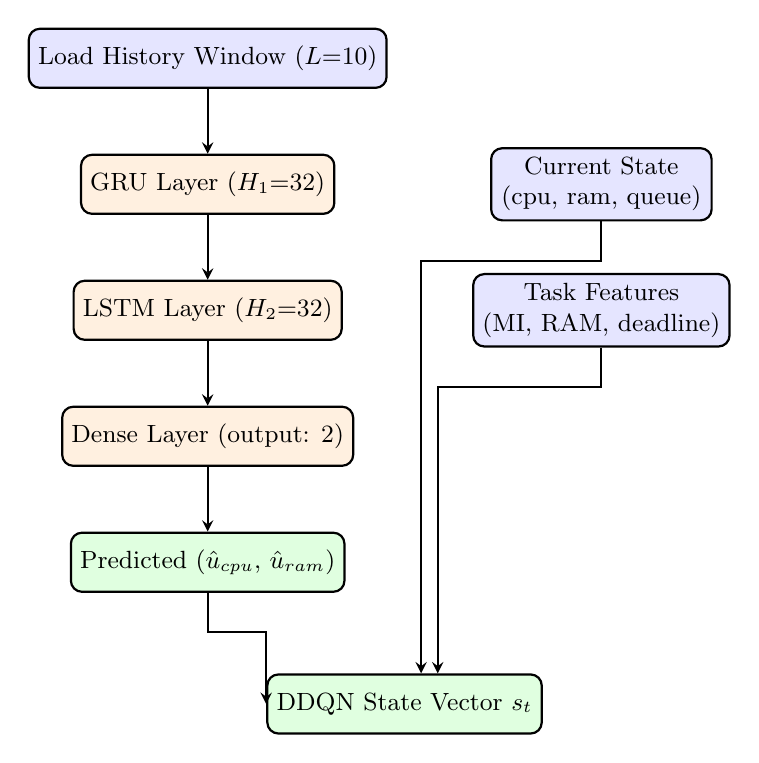
\begin{tikzpicture}[>=stealth, thick, font=\small]

\tikzstyle{block}  = [rectangle, draw, rounded corners,
                       fill=blue!10, minimum width=2.8cm,
                       minimum height=0.75cm, align=center]
\tikzstyle{proc}   = [rectangle, draw, rounded corners,
                       fill=orange!12, minimum width=2.8cm,
                       minimum height=0.75cm, align=center]
\tikzstyle{outbox} = [rectangle, draw, rounded corners,
                       fill=green!12, minimum width=2.8cm,
                       minimum height=0.75cm, align=center]

% ── Left column: predictor chain ──────────────────────
\node[block]  (hist)  at (0, 0)    {Load History Window ($L{=}10$)};
\node[proc]   (gru)   at (0,-1.6)  {GRU Layer ($H_1{=}32$)};
\node[proc]   (lstm)  at (0,-3.2)  {LSTM Layer ($H_2{=}32$)};
\node[proc]   (dense) at (0,-4.8)  {Dense Layer (output: 2)};
\node[outbox] (pred)  at (0,-6.4)  {Predicted $(\hat{u}_{\text{cpu}},\,\hat{u}_{\text{ram}})$};

% ── Right column: context inputs ──────────────────────
\node[block]  (curr)  at (5, -1.6) {Current State\\(cpu, ram, queue)};
\node[block]  (task)  at (5, -3.2) {Task Features\\(MI, RAM, deadline)};

% ── Output: state vector ──────────────────────────────
\node[outbox] (state) at (2.5,-8.2) {DDQN State Vector $s_t$};

% ── Arrows: left chain ───────────────────────────────
\draw[->] (hist)  -- (gru);
\draw[->] (gru)   -- (lstm);
\draw[->] (lstm)  -- (dense);
\draw[->] (dense) -- (pred);

% ── Arrows: converge to state vector ─────────────────
\draw[->] (pred.south)  -- ++(0,-0.5) -| (state.west);
\draw[->] (curr.south)  -- ++(0,-0.5) -| ([xshift=6pt]state.north);
\draw[->] (task.south)  -- ++(0,-0.5) -| ([xshift=12pt]state.north);

\end{tikzpicture}
\caption{GRU-LSTM Predictor Pipeline: historical load window
         passes through GRU and LSTM layers to produce next-step
         utilisation forecasts, which are concatenated with
         current state and task features to form the DDQN
         state vector $s_t$.}
\label{fig:lstm_pipeline}
\end{figure}

\subsection{GRU Update Equations}

At each time step $t$ in the window, the GRU hidden state is
updated as:
\begin{equation}
  z_t = \sigma(W_z x_t + U_z h_{t-1} + b_z)
  \label{eq:gru_update}
\end{equation}
\begin{equation}
  r_t = \sigma(W_r x_t + U_r h_{t-1} + b_r)
  \label{eq:gru_reset}
\end{equation}
\begin{equation}
  \tilde{h}_t = \tanh(W_h x_t + U_h (r_t \odot h_{t-1}) + b_h)
  \label{eq:gru_candidate}
\end{equation}
\begin{equation}
  h_t^{\text{GRU}} = (1 - z_t) \odot h_{t-1} + z_t \odot \tilde{h}_t
  \label{eq:gru_hidden}
\end{equation}
where $z_t$ and $r_t$ are the update and reset gates, $\sigma$ is
the sigmoid function, and $\odot$ denotes element-wise
multiplication.

\subsection{LSTM Update Equations}

The output $h_L^{\text{GRU}}$ of the GRU layer is fed as input
to the LSTM layer:
\begin{equation}
  f_t = \sigma(W_f [h_{t-1}^{\text{LSTM}}, h_t^{\text{GRU}}] + b_f)
  \label{eq:lstm_forget}
\end{equation}
\begin{equation}
  i_t = \sigma(W_i [h_{t-1}^{\text{LSTM}}, h_t^{\text{GRU}}] + b_i)
  \label{eq:lstm_input}
\end{equation}
\begin{equation}
  \tilde{c}_t = \tanh(W_c [h_{t-1}^{\text{LSTM}}, h_t^{\text{GRU}}] + b_c)
  \label{eq:lstm_cell_candidate}
\end{equation}
\begin{equation}
  c_t = f_t \odot c_{t-1} + i_t \odot \tilde{c}_t
  \label{eq:lstm_cell}
\end{equation}
\begin{equation}
  o_t = \sigma(W_o [h_{t-1}^{\text{LSTM}}, h_t^{\text{GRU}}] + b_o),
  \quad h_t^{\text{LSTM}} = o_t \odot \tanh(c_t)
  \label{eq:lstm_output}
\end{equation}

\subsection{Predictor Training}

Each per-cloudlet predictor is pre-trained on 500 episodes of
simulated load traces using the Mean Squared Error (MSE) loss:
\begin{equation}
  \mathcal{L}_{\text{pred}}
  = \frac{1}{B} \sum_{b=1}^{B}
    \bigl\| \hat{\mathbf{y}}_b - \mathbf{y}_b \bigr\|_2^2
  \label{eq:pred_loss}
\end{equation}
where $B$ is the mini-batch size and $\mathbf{y}_b$ is the ground
truth next-step utilisation vector. Training uses the Adam
optimiser with learning rate $10^{-3}$ for 20 epochs. After
pre-training, the predictor weights are frozen and the network
operates in inference mode throughout DDQN training.

% ─────────────────────────────────────────────────────────
\section{State, Action, and Reward Design}
\label{sec:sar}

\subsection{State Vector Construction}

At each step $t$, the broker assembles the state vector
$s_t \in \mathbb{R}^{6N+5}$ by concatenating:
\begin{equation}
  s_t = \bigl[
    \underbrace{\mathbf{o}_1, \ldots, \mathbf{o}_N}_{\text{current state}},\;
    \underbrace{\hat{\mathbf{y}}_1, \ldots, \hat{\mathbf{y}}_N}_{\text{LSTM forecasts}},\;
    \underbrace{\mathbf{f}_\tau}_{\text{task features}},\;
    \underbrace{g, \text{JFI}}_{\text{global}}
  \bigr]
  \label{eq:state_vec}
\end{equation}
where $\mathbf{o}_i = (\text{cpu\_util}_i,\, \text{ram\_util}_i,\,
q_i / K_i)$ is the current resource observation for cloudlet $i$,
$\hat{\mathbf{y}}_i = (\hat{u}_{\text{cpu},i},
\hat{u}_{\text{ram},i})$ is the GRU-LSTM forecast,
$\mathbf{f}_\tau = (\text{MI}/\text{MI}_{\max},\,
r_\tau/R_{\max},\, d_\tau/d_{\max})$ encodes the arriving task,
$g$ is the mean CPU utilisation across all cloudlets, and JFI is
Jain's Fairness Index defined as:
\begin{equation}
  \text{JFI} = \frac{\left(\sum_{i=1}^{N}
    \text{cpu\_util}_i\right)^2}
    {N \sum_{i=1}^{N} \text{cpu\_util}_i^2}
  \label{eq:jfi}
\end{equation}

\subsection{Action Space}

The discrete action $a_t \in \{0, 1, \ldots, N\}$ selects the
destination for the arriving task. Actions $0$ to $N{-}1$
correspond to the $N$ edge cloudlets; action $N$ routes to the
cloud. For the 3-cloudlet topology $|\mathcal{A}| = 4$.

\subsection{Reward Function}

The scalar reward at step $t$ is a weighted sum of six terms:
\begin{equation}
  r_t = w_1 r_{\text{drop}} + w_2 r_{\text{lat}}
      + w_3 r_{\text{dl}}   + w_4 r_{\text{energy}}
      + w_5 r_{\text{bal}}  + w_6 r_{\text{over}}
  \label{eq:reward_method}
\end{equation}

\begin{itemize}
  \item $r_{\text{drop}} = -1$ if task dropped, else $0$.
  \item $r_{\text{lat}} = -l_i / l_{\max}$, latency penalty.
  \item $r_{\text{dl}} = -1$ if $l_i > d_\tau$, else $0$.
  \item $r_{\text{energy}} = -e_i / e_{\max}$, energy penalty.
  \item $r_{\text{bal}} = \text{JFI}(t) - 1 \in [-1, 0]$,
  where $\text{JFI}(t) \in (0, 1]$ so this term is always
  non-positive.
  \item $r_{\text{over}} = -\mathbf{1}[\text{cpu\_util}_{a_t} > 0.62]$.
\end{itemize}

The weights $(w_1, \ldots, w_6) = (5, 1, 2, 0.5, 1, 2)$ are set
so that drop reduction is the primary objective and balance and
overload prevention act as regularisation. All reward components
are non-positive; this all-penalty formulation is deliberate —
the agent maximises cumulative reward by minimising total
penalty, which is equivalent to jointly minimising drops,
latency, energy, and imbalance. No explicit positive reward
is needed because the improvement signal comes from the
\emph{relative difference} between penalty levels across actions.

% ─────────────────────────────────────────────────────────
\section{Stage 2: Double Deep Q-Network Agent}
\label{sec:ddqn}

\subsection{Network Architecture}

The DDQN agent comprises two networks with identical architecture:
the \emph{online network} $Q(s, a;\, \theta)$ and the
\emph{target network} $Q(s, a;\, \theta^-)$. Each network is a
four-layer multi-layer perceptron (MLP):
\begin{equation}
  \text{Layer sizes:} \quad
  (6N{+}5) \rightarrow 256 \rightarrow 256 \rightarrow 128 \rightarrow |\mathcal{A}|
  \label{eq:network_arch}
\end{equation}
ReLU activations follow each hidden layer. The output layer
produces $|\mathcal{A}|$ Q-values with no activation.

\subsection{Double DQN Loss}

Standard DQN tends to overestimate Q-values because it uses the
same network to select and evaluate the greedy action. DDQN
separates these two roles:
\begin{equation}
  a^* = \arg\max_{a} Q(s_{t+1}, a;\, \theta)
  \label{eq:ddqn_action_select}
\end{equation}
\begin{equation}
  y_t^{\text{DDQN}} = r_t + \gamma \,
    Q(s_{t+1}, a^*;\, \theta^-)
  \label{eq:ddqn_target}
\end{equation}
\begin{equation}
  \mathcal{L}(\theta) = \mathbb{E}_{(s,a,r,s') \sim \mathcal{D}}
  \!\left[
    \bigl( y_t^{\text{DDQN}} - Q(s_t, a_t;\, \theta) \bigr)^2
  \right]
  \label{eq:ddqn_loss}
\end{equation}
where $\mathcal{D}$ is the experience replay buffer and
$\theta^-$ is updated by copying $\theta$ every
$C_{\text{update}} = 200$ steps.

\subsection{$\varepsilon$-Greedy Exploration}

During training the agent follows an $\varepsilon$-greedy policy:
\begin{equation}
  \pi_\varepsilon(s) =
  \begin{cases}
    \text{random action} & \text{with probability } \varepsilon \\
    \arg\max_a Q(s,a;\theta) & \text{with probability } 1-\varepsilon
  \end{cases}
  \label{eq:eps_greedy}
\end{equation}
$\varepsilon$ decays linearly from 1.0 to 0.05 over the first
500 episodes, then remains at 0.05.

% ─────────────────────────────────────────────────────────
\section{PPO Baseline Agent}
\label{sec:ppo}

A Proximal Policy Optimisation (PPO) agent is trained as a
baseline using the same state space, action space, and reward
function as DDQN. PPO clips the probability ratio between the old
and updated policy to prevent destructive updates:
\begin{equation}
  \mathcal{L}^{\text{CLIP}}(\phi) = \mathbb{E}_t \!\left[
    \min\!\left(
      \rho_t(\phi)\, \hat{A}_t,\;
      \text{clip}(\rho_t(\phi),\, 1{-}\epsilon,\, 1{+}\epsilon)\,
      \hat{A}_t
    \right)
  \right]
  \label{eq:ppo_clip}
\end{equation}
where $\rho_t(\phi) = \pi_\phi(a_t|s_t)/\pi_{\phi_{\text{old}}}
(a_t|s_t)$ is the probability ratio and $\hat{A}_t$ is the
generalised advantage estimate. The clipping parameter
$\epsilon = 0.2$ and the discount $\gamma = 0.99$ are used. PPO
serves as the primary on-policy comparison to verify the
sample-efficiency advantage of DDQN.

% ─────────────────────────────────────────────────────────
\section{Training Procedure}
\label{sec:training}

\subsection{Algorithm: DRL-LSTM-LBRO Training}

\begin{algorithm}[htbp]
\caption{DRL-LSTM-LBRO Training Procedure}
\label{alg:training}
\begin{algorithmic}[1]
\Require Episodes $E$, steps per episode $T$, replay buffer
         $\mathcal{D}$, batch size $B$, target update interval
         $C$, pre-trained GRU-LSTM predictors $\{\Phi_i\}$
\Ensure Trained DDQN parameters $\theta$

\State Initialise $\theta$ randomly; $\theta^- \leftarrow \theta$
\State Initialise $\mathcal{D}$ with capacity 50{,}000
\State $\varepsilon \leftarrow 1.0$

\For{episode $e = 1$ to $E$}
  \State Reset environment; observe initial state $s_0$
  \For{step $t = 0$ to $T-1$}
    \State Obtain GRU-LSTM forecasts $\hat{\mathbf{y}}_i \leftarrow \Phi_i(\mathbf{X}_i^{(t)})$ for each cloudlet $i$
    \State Construct state $s_t$ via Equation~(\ref{eq:state_vec})
    \State Sample action $a_t$ via $\varepsilon$-greedy policy (Eq.~\ref{eq:eps_greedy})
    \State Execute $a_t$; observe reward $r_t$ and next state $s_{t+1}$
    \State Store $(s_t, a_t, r_t, s_{t+1})$ in $\mathcal{D}$
    \If{$|\mathcal{D}| \geq B$}
      \State Sample mini-batch of $B$ transitions from $\mathcal{D}$
      \State Compute DDQN targets via Equations~(\ref{eq:ddqn_action_select})--(\ref{eq:ddqn_target})
      \State Update $\theta$ by minimising $\mathcal{L}(\theta)$ (Eq.~\ref{eq:ddqn_loss})
    \EndIf
    \If{$t \bmod C = 0$}
      \State $\theta^- \leftarrow \theta$
    \EndIf
  \EndFor
  \State Decay $\varepsilon$
\EndFor
\State \Return $\theta$
\end{algorithmic}
\end{algorithm}

\subsection{Algorithm: Task Placement at Inference}

\begin{algorithm}[htbp]
\caption{DRL-LSTM-LBRO Task Placement (Inference)}
\label{alg:inference}
\begin{algorithmic}[1]
\Require Arriving task $\tau$, trained $\theta$, predictors
         $\{\Phi_i\}$, cloudlet set $\mathcal{C}$

\State Obtain forecasts $\hat{\mathbf{y}}_i \leftarrow \Phi_i(\mathbf{X}_i)$ for all $i$
\State Construct state $s$ via Equation~(\ref{eq:state_vec})
\State $a^* \leftarrow \arg\max_a Q(s, a;\, \theta)$

\If{$a^* \in \{0, \ldots, N{-}1\}$}   \Comment{edge cloudlet selected}
  \If{$q_{a^*} < K_{a^*}$ \textbf{and}
      $\text{ram\_util}_{a^*} \cdot R_{a^*} + r_\tau \leq R_{a^*}$}
    \State Accept $\tau$ at cloudlet $a^*$
  \Else
    \State Offload $\tau$ to cloud   \Comment{capacity constraint violated}
  \EndIf
\Else
  \State Offload $\tau$ to cloud
\EndIf
\end{algorithmic}
\end{algorithm}

\subsection{Hyperparameter Summary}

Table~\ref{tab:hyperparams} lists all key hyperparameters used
during training.

\begin{table}[htbp]
\centering
\caption{Training Hyperparameters}
\label{tab:hyperparams}
\renewcommand{\arraystretch}{1.15}
\begin{tabular}{lcc}
\toprule
\textbf{Parameter} & \textbf{DDQN} & \textbf{PPO} \\
\midrule
Hidden layer sizes        & 256--256--128 & 256--256--128 \\
Learning rate             & $5 \times 10^{-4}$ & $3 \times 10^{-4}$ \\
Discount $\gamma$         & 0.99 & 0.99 \\
Replay buffer size        & 50{,}000 & --- \\
Mini-batch size $B$       & 64 & 64 \\
Target update interval $C$& 200 steps & --- \\
$\varepsilon$ start/end   & 1.0 / 0.05 & --- \\
Clip parameter $\epsilon$ & --- & 0.2 \\
Optimiser                 & Adam & Adam \\
Episodes $E$              & 1{,}000 & 1{,}000 \\
Steps per episode $T$     & 2{,}000 & 2{,}000 \\
GRU-LSTM window $L$       & 10 & 10 \\
\bottomrule
\end{tabular}
\end{table}
